%
% $RCSfile: waterfall_process.tex,v $
%
% Copyright (C) 2002-2008. Christian Heller.
%
% Permission is granted to copy, distribute and/or modify this document
% under the terms of the GNU Free Documentation License, Version 1.1 or
% any later version published by the Free Software Foundation; with no
% Invariant Sections, with no Front-Cover Texts and with no Back-Cover
% Texts. A copy of the license is included in the section entitled
% "GNU Free Documentation License".
%
% http://www.cybop.net
% - Cybernetics Oriented Programming -
%
% http://www.resmedicinae.org
% - Information in Medicine -
%
% Version: $Revision: 1.1 $ $Date: 2008-08-19 20:41:09 $ $Author: christian $
% Authors: Christian Heller <christian.heller@tuxtax.de>
%

\section{Waterfall Process}
\label{waterfall_process_heading}
\index{Waterfall Process}
\index{Requirements}
\index{Analysis}
\index{Design}
\index{Implementation}
\index{Test}
\index{Integration}
\index{Back Flow of Waterfall Process}
\index{V-Model}
\index{V-Modell 97}
\index{Big Bang Delivery}

The \emph{Waterfall Process} (figure \ref{waterfall_figure}) is the classical
way to develop a product. It assumes that the requirements are clear and do not
change during a project. Waterfall software development is pretty straightforward
and usually consists of the sequenced phases \emph{Requirements}, \emph{Analysis},
\emph{Design}, \emph{Implementation} (Realisation, Coding), \emph{Test} and
\emph{Integration} (Release).

\begin{figure}[ht]
    \begin{center}
        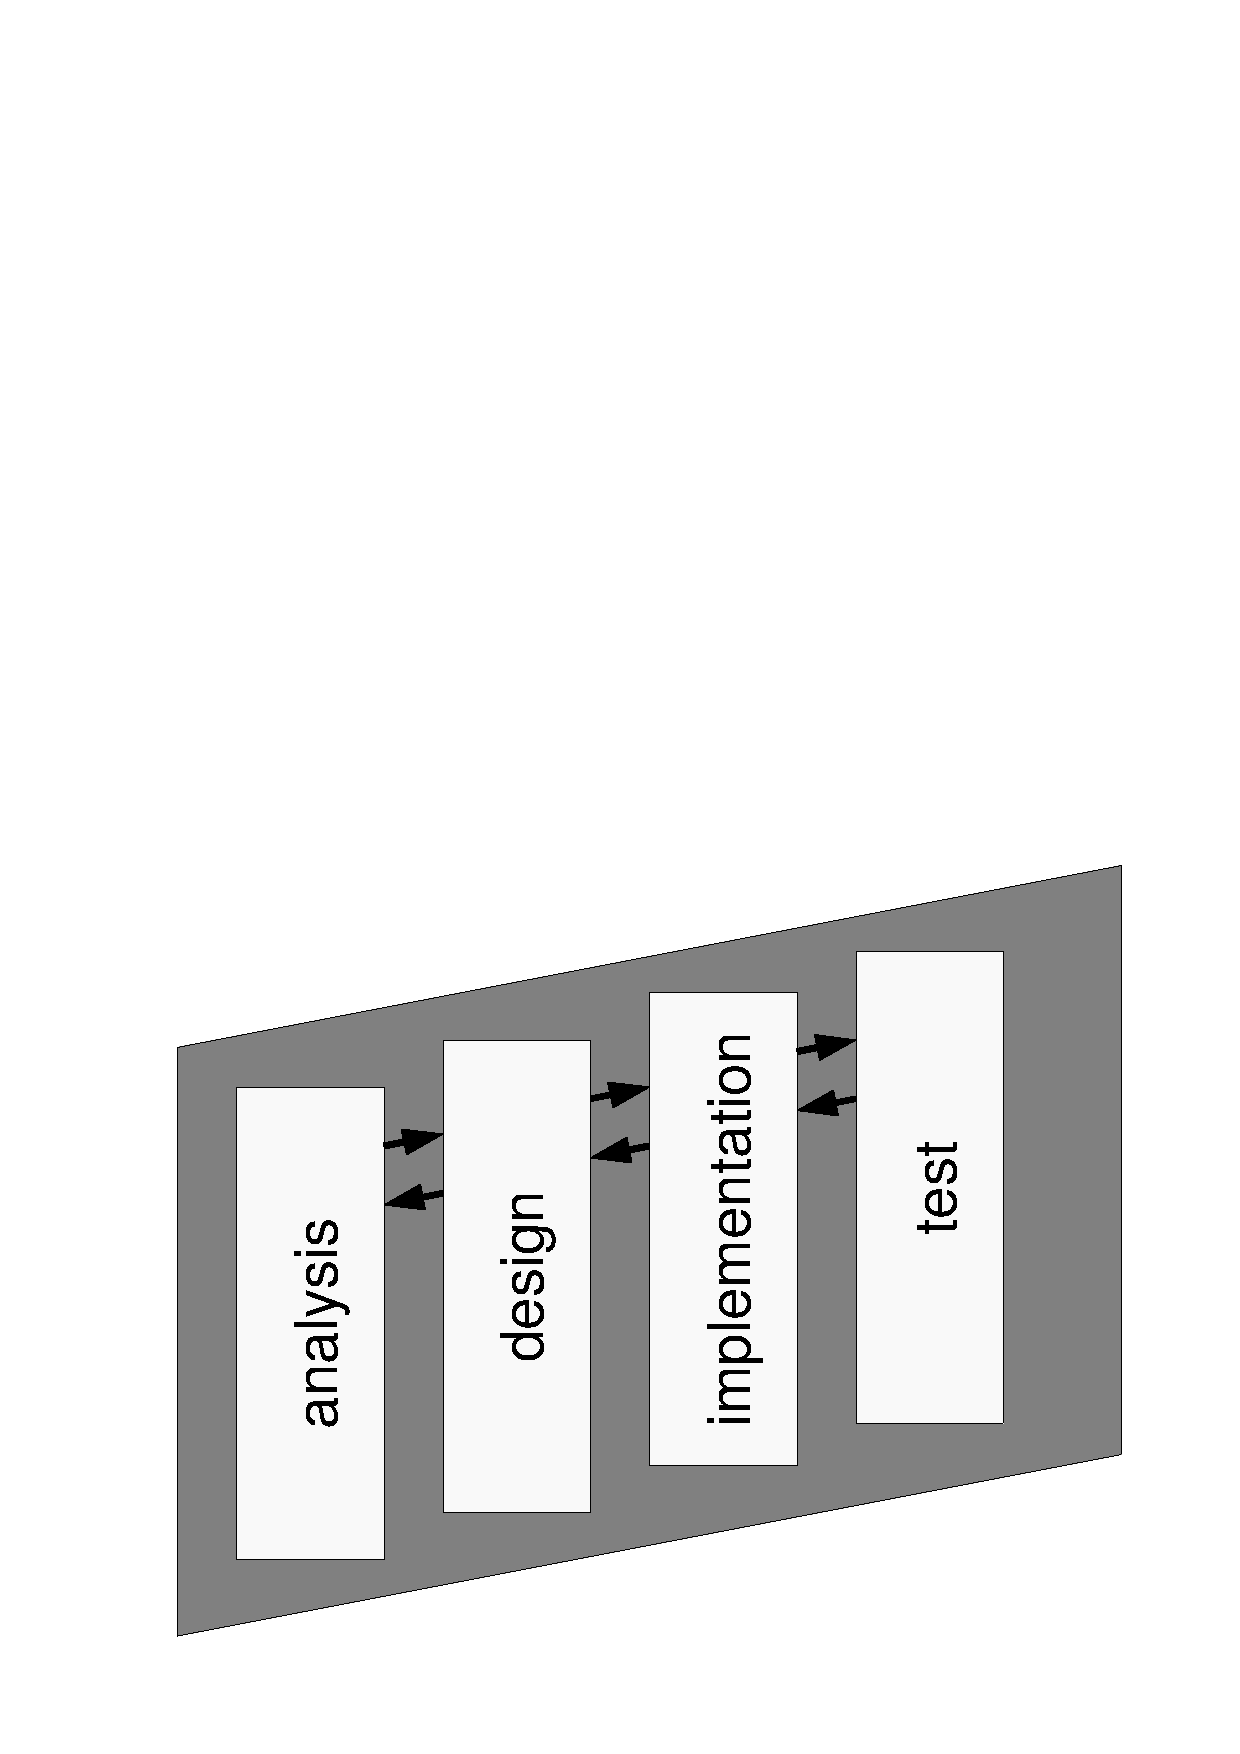
\includegraphics[scale=0.3,angle=-90]{graphic/waterfall.pdf}
        \caption{Waterfall Process with Back Flow}
        \label{waterfall_figure}
    \end{center}
\end{figure}

\begin{figure}[ht]
    \begin{center}
        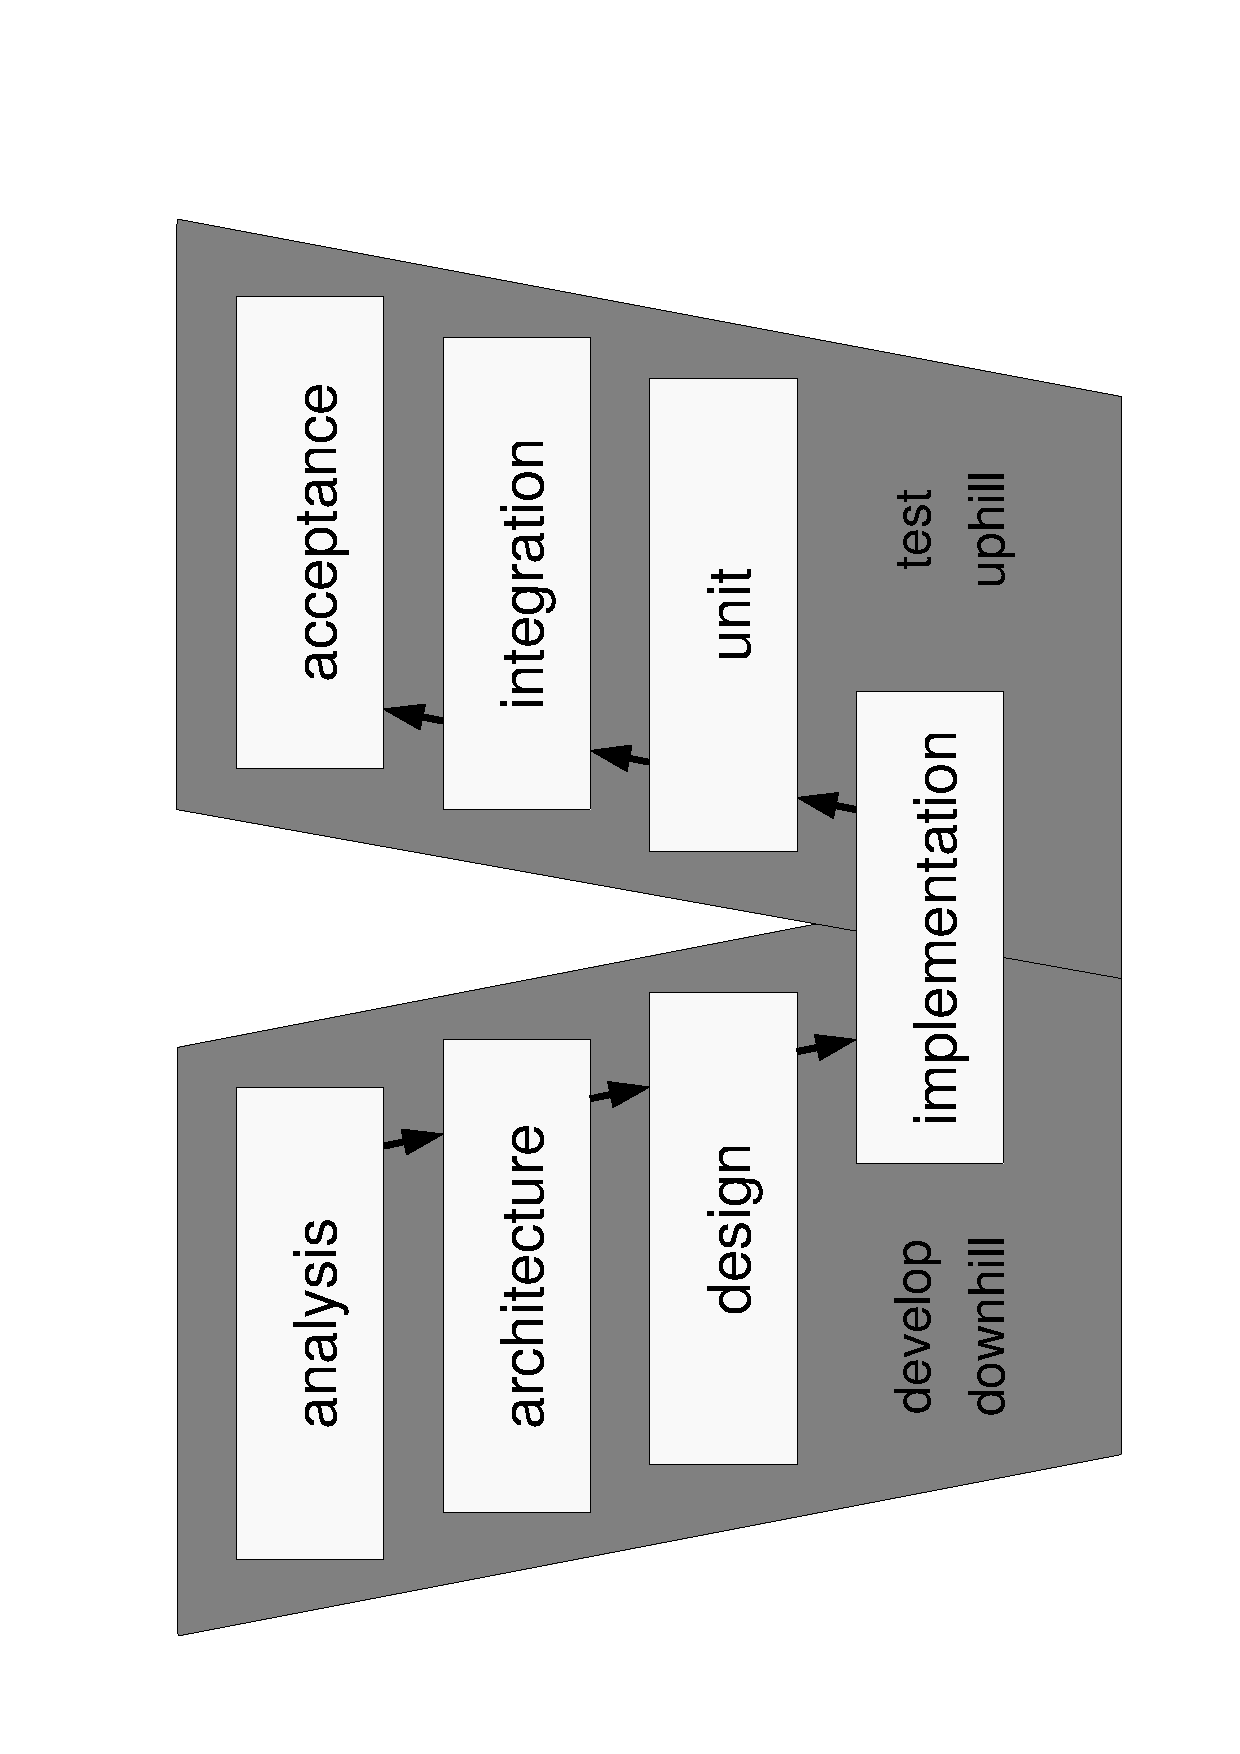
\includegraphics[scale=0.3,angle=-90]{graphic/vmodel.pdf}
        \caption{V-Model}
        \label{vmodel_figure}
    \end{center}
\end{figure}

Numerous variations of waterfall processes exist. The simplest ones deliver
their product at once, at the end of the project, what is often called
\emph{Big Bang Delivery} \cite{malotaux}. Others integrate some kind of
\emph{Back Flow} \cite{sweedyk} that allows to consider test results in further
development. One example that has combined software development- and testing
activities is the \emph{V-Modell 97} \cite{vmodel} (figure \ref{vmodel_figure}).
Its name stands for its shape: the left-hand (downhill) side of the \emph{V}
represents the development; the right-hand (uphill) side represents the
corresponding test activities.
